\chapter{Introduction}
\label{chap-intro}

Physics is to study matters of the universe where 
there are tremendous more disordered materials than ordered ones.
In ordered physics, there has been a rich spectrum of 
well-defined theories, models, phases, and methods; while disordered 
systems still have a variety of challenging and unclear questions. 

This chapter first introduces the general disordered system and 3 specific disordered systems, i.e. jamming transition, antiferromagnetic Ising model, and random field Ising model. Then the finite dimensional networks we use in our study are described. In the end of this chapter, the computational methods used are reviewed and discussed.

\section{Disordered System}
In the real world, most materials can be considered as disordered materials because of their heterogeneous structures with defects and impurities. While the techniques to study and understand the properties of ordered materials are well-developed, our
ability to anticipate, let alone to design, properties of disordered materials have not yet reached nearly the same level of sophistication \cite{Kotani16Material}. 

Disordered materials not only have the most amount but also numerous categories or types. There are various types of disordered materials, such as glass \cite{Gibbs1958nature, berthier2016facets}, amorphous solids \cite{berthier2016facets}, polymer s\cite{roth2005glass}, granular materials \cite{richard2005slow}, and biological tissues \cite{bi2015density}. 

Here we focus on models of disordered systems that lend themselves to theoretical investigations, such as Edwards-Anderson model \cite{edwards1975theory}, Sherrington-Kirkpatrick model \cite{sherrington1975}, random field Ising model (RFIM) \cite{imry1975random}, antiferromagnetic Ising model (AFM) \cite{wannier1950afm},  fully frustrated model \cite{kosterlitz1973ordering, kosterlitz1974critical}, spin glass \cite{young1997spin}, lattice glass model \cite{Biroli02}. These different models share  three main similarities. 
\begin{figure}[h]
\centering 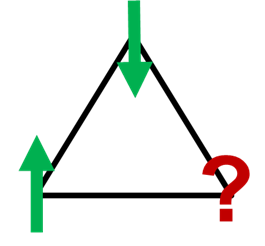
\includegraphics[width=0.2\columnwidth]{Chapter-1/geo_frustration.png} 
\protect\caption{\label{fig:intro-gf} An example of the geometric frustration in antiferromagnetic Ising model. There are more than one ground states even in this simple triangular lattice. A more complex network would lead to extensive frustrations.}
\end{figure}

Two main commonalities are frustrations (from geometry or quenched disorder) and glassy dynamics  in these systems. First, the frustration is usually introduced either by  random interactions (quenched disorder) or complex structures \cite{vannimenus1977}. For example, in AFM, any odd loop in the structure can lead to the geometric frustration \cite{wannier1950afm} (as illustrated by Fig. \ref{fig:intro-gf}). In spin glass, the interaction constant $J_{ij}$ between spin $i$ and $j$ is random and can be either negative or positive, which is known as frustrated interaction \cite{edwards1975theory} or quenched disorder.
Second, the glassy dynamics is often observed in the simulations of these disordered systems \cite{lunkenheimer2000}. For example, a strongly interacting glassy material is observed to have a power-law relaxation \cite{palmer1984}. The glassy dynamics often lead to the glass transition \cite{biroli2013perspective} or jamming transition \cite{Liu1998}. 
In all the three disordered systems studied (Chapter 2 - 4), they share both the geometric frustration and the glassy dynamics with a power-law relaxation, and we explore to see whether there is any phase transition or glass transition.

Another commonality is the analytical and computational complexity. Analytically, only certain models in certain lattices or structures are exactly solvable. For example, the mean field theory  \cite{kadanoff2009} is the most popular method to solve problems of spin glass \cite{sherrington1975}, lattice glass model \cite{Biroli02}, fully frustrated XY model \cite{kim2001xy}, etc. However, the majority of these models in real-world lattice or complex networks are not analytically solvable. Moreover, their computational complexity is often NP-complete \cite{garey1983} because the computational cost grows exponentially with the system size \cite{barahona1982, weigt2000}. These difficulties of computational complexity drive physicists to develop efficient and robust methods and algorithms to solve the problems in disordered systems, and these methods and algorithms go even beyond physics  \cite{mezard1990spin, stein2013spin}.

In our studies, we have the same difficulties. In order to address these problems, we utilize a combination \cite{cheng2015jamming, ma2016prb} of real-world-like lattices, Monte Carlo methods, and an analytical method RG using scientific computing languages (C/C++, Python) and modern computing tools (Mathematica, MATLAB). Our physical modeling, computational implementations, and results are described in details in Chapters 2-4.


\section{Jamming Transition}
\label{sec:jam_intro}
The first focus here is on the jamming systems \cite{Biroli2007}. Those systems undergo 
a jamming transition from a liquid-like to a solid-like state with extremely slow 
dynamics at a high packing density. The most interesting part in this 
disordered system is the physics near the jamming transition. 
The jamming transition, as discussed by Liu and
Nagel in 1998~\cite{Liu1998} has been the focus of
intense study~\cite{Biroli2007,Liu2010,Berthier2011}. 

A granular disordered system with increasing density can reach a jammed state at which a finite yield stress develops, or at least extremely long relaxation times
ensue, similar to the emerging sluggish behavior observed when the
viscosity of a cooled glassy liquid seemingly diverges. Thus, a jamming
transition may be induced in various ways, such as by increasing density,
decreasing temperature, or/and reducing shear stress~\cite{Liu2010}.
Below the jamming transition, the system stays in long-lived meta-stable
states, and its progression to its corresponding equilibrium state
entails an extremely slow, non-Debye relaxation~\cite{Hill1985, Ciamarra2010, van2010}.

Jamming transitions have been observed in various types of systems,
such as granular media~\cite{Majmudar2007}, molecular glasses~\cite{Parisi2010,Angelani2007},
colloids~\cite{Trappe2001}, emulsions~\cite{Zhang2005}, foams~\cite{Berthier2011,DaCruz2002},
etc~\cite{Liu2010,van2010}. These systems can behave like stiff solids
at a high density with low temperature and small perturbations. In
these transitional processes, the systems can self-organize their
own structure to avoid large fluctuations~\cite{Berthier2011} and
to reach a quasi-stable jammed state, characterized by an extremely
slow evolution to the unjammed equilibrium state. The properties of
those quasi-stable non-equilibrium states as well as their corresponding
equilibrium state is the main focus of our work in jamming. 


The properties of the jamming transition have been studied 
extensively~\cite{Biroli2007,Majmudar2007,Liu2010}, but we still lack an essential
understanding of the physics underlying the jammed state. Theoretical
progress has been much slower than the accumulation of experimental
discoveries. One of the reasons is the scarcity of theoretical microscopic
models to capture the complex jamming process~\cite{Krzakala2008,Jacquin2011}. 

In recent years, a lattice glass model proposed by Biroli and Mezard
(BM)~\cite{Biroli02} has been shown as a simple but adequate means
to study the jamming process. It is simple because the model follows
specific dynamical rules which are elementary to implement in both
simulations and analytical work. In distinction to kinetically constrained
models such as that due to Kob and Andersen~\cite{Kob93}, in which
particles are blocked from leaving a position unless certain neighborhood
conditions are satisfied, BM embeds geometric frustration merely by
preventing the neighborhood of any particles to consist of more than
$l$ other particles. Beyond that, it proceeds purely thermodynamically.
The phase diagram can be reduced to just one (or both) of two control
parameters, chemical potential and temperature. Either is sufficient
to reproduce a jamming transition which is similar to that observed
in off-lattice systems~\cite{Biroli02}. 

Using this model in a mean-field network 
(i.e., a regular random graph), Krzakala \textit{et al.} find
jammed states in Monte Carlo simulations and a genuine thermodynamical
phase transition (ideal glass transition) in its mean-field analytical
solutions~\cite{Krzakala2008}. In other words, the jammed state coincides
with an underlying equilibrium state that possesses a phase transition
to a glassy state. There is also other work trying to prove the similar idea using mean-field models \cite{Rivoire03,berthier2011theory, Parisi2010}. That raises the prospect that this equilibrium phase transition might be the reason for the onset of jamming. However, such a connection between phase transition and jamming transition is hard to ascertain for finite-dimensional lattice glasses. Our work (Chapter \ref{chap-jamming}) focuses on jamming in finite-dimensional hierarchical networks which could contribute closer insights to real world systems.



\section{Ising models}
The Ising model was proposed by Wilhelm Lenz and Ernst Ising \cite{ising1925contribution, brush1967history} in the 1920s. It has simple nearest-neighbor interactions and a simple Hamiltonian (energy)
\begin{equation}
\mathcal{H}=-J \sum_{\langle i, j\rangle}^N s_i s_j - H \sum_{i=1}^N s_i
\label{eq:intro-ising}
\end{equation}
where $s_i=\pm1$, $\langle i, j\rangle$ stands for nearest-neighbor spin-pair, $s_i$ $J$ ($>0$)is the exchange interaction constant, and $H$ is the external magnetic field. This is the most simple Ising model and usually called ferromagnetic Ising model (FM).
However, this simple model could represent approximately real-world systems and lead to phase transitions \cite{onsager1944} or complex dynamics \cite{Fredrickson1984} in different lattice structures. 
Numerous variations have been proposed to study different systems, ranging from magnetic systems \cite{blundell2001magnetism} to biological systems \cite{hopfield1982neural}.

In this section, two disordered Ising models, antiferromagnetic Ising model and random field Ising model,  are introduced and reviewed. They are also the focus of the studies in Chapter \ref{chap-afm} and Chapter \ref{chap-rfim}.


\subsection{Antiferromagnetic Ising Model}
\label{sec:intro-afm}
Unlike ferromagnetic Ising model (FM) having a large amount of investigations \cite{niss2005history, mccoy2014two}, the antiferromagnetic Ising model (AFM) have little work published until the 1970s \cite{penney2003new}. The most interesting characteristic of the AFM is that it can easily introduce geometric frustrations and may give rise to a glassy dynamics or even spin glass phase. While this interesting characteristic is realized by simply changing the sign of the coupling constant $J$ ($J<0$), and the Hamiltonian is still the same as in Eq. \ref{eq:intro-ising}. Then the geometric frustrations can be simply introduced through odd loops (as illustrated in Fig. \ref{fig:intro-gf}).

Using a combination of the simple AFM and complex networks, there has been interesting phenomena observed, such as glassy dynamics \cite{shokef2011}, magnetization plateaus \cite{ohanyan2003mag}, and spin glass phase transition \cite{herrero2008afm}. However, most results have been gained from the exact solution of such models in their mean-field
approximation, and these mean-field descriptions for disordered systems often fail to capture the properties of real, finite-dimensional materials.  Unlikely most of these findings, we study the AFM in real-world lattice-like Hanoi networks who remain exactly renormalizable. Through these methods, we can learn both the non-equilibrium and equilibrium behaviors. 

Our work using the AFM is inspired by an early attempt in Ref. \cite{mckay1982spin} to avoid randomness with a family of geometrically frustrated hierarchical networks susceptible to an exact renormalization group (RG) treatment. As there, we find that glassy behavior is associated
with a transition into chaos for the RG-flow in coupling space. We
show that this transition into the glass state is of infinite order
and occurs via a sub-critical Hopf-bifurcation in the RG-flow \cite{weinrib1983critical}.
This chaotic flow appears as a natural manifestation of temperature
chaos that is a characteristic of glassy order  \cite{bray1987chaotic, thomas2011zero}.
We study the scaling behavior of the zero-crossings in the domain-wall
free-energy, for which we can derive an exact expression in terms
of renormalized couplings. More details are described in Sec. \ref{sec:afm-rg}.



\subsection{Random Field Ising Model}
\label{sec:intro-rfim}
The random field Ising model (RFIM) was first introduced by Imry and Ma \cite{imry1975random} in 1975. It represents a class of quenched disordered spin models \cite{young1997spin} with  disorderedness coupled to the each spin, which is different from the spin glass models with disordered interaction constants. The general Hamiltonian of RFIM with $N$ spins is
\begin{equation}
\mathcal{H}=-J\sum_{<i,j>}s_{i}s_{j}-\sum_{i=1}^{N}h_{i}s_{i}
\end{equation}
where the major difference from traditional Ising model is the random field term $h_i$ for spin $i$. Different spins usually have  identical independent distributed random fields $h_i$, and $h_i$ often follows a uniform \cite{nattermann1997theory} or Gaussian distribution \cite{newman1999}.

As a statistical mechanical model, the most investigated theoretical aspect of RFIM is still the critical phenomena, such as ferromagnetic phase transition. For one dimensional RFIM, its exact solution suggests no phase transition \cite{grinstein1983exact}. Through a number of theoretical calculations \cite{parisi1979random, bricmont1987lower}, three dimensional RFIM has a phase transition from a paramagnetic phase to a ferromagnetic one  \cite{bricmont1987lower}, which suggests the lower critical dimension is $d_l = 3$. 

However, the focus of our study in Chapter \ref{chap-rfim} is not the phase transition but the aging dynamics of the RFIM simulating experimental system. In terms of experimental studies, the diluted antiferromagnet is considered as an experimental realization of the RFIM \cite{belanger1985, fernandez1988random}. It has also been used to study other materials, such as  impure substrates \cite{villain1982commensurate}, and magnetic alloys \cite{fisher1988theory}. 
The experimental system to model here is a thin-film ferromagnet/antiferromagnet bilayer which exhibits non-Arrhenius power-law aging of the magnetization state \cite{ma2016prb}. 
It is expected that, in such a complex experimental magnetic system, the aging or relaxation to equilibrium state may be trapped by metastable states, and the relaxation may follow an exponential scaling according to the Arrhenius law \cite{Arrhenius1989}
\begin{equation}
\tau = \tau_0 \exp \left( \frac{E}{k_B T}\right)
\end{equation}
where $\tau$ is the characteristic activation time, $\tau_0$ is a material-dependent pre-exponential factor, $E$ is the energy barrier between two local/local (or local/global) minimum, $k_B$ is the Boltzmann constant, and $T$ is the temperature. However, what is observed in the experiment is a power-law relaxation with a subunity exponent instead of exponential relaxation. The experiment itself cannot explain this phenomena, and the small exponent is not convincing either to conclude the power-law relaxation. 

In order to explain the experiment and justify the small-exponent power-law, we use a two dimensional RFIM and the Monte Carlo method to simulate the experimental material with simplifying approximations. This simple model captures the salient features of the non-Arrhenius aging observed in the experimental measures, i.e., power-law relaxation with a subunity exponent. In addition to the scaling, the aging in the Monte Carlo simulation can be easily visualized, which shows the system evolves to two big domains with oppositely oriented spins. What the aging can do is actually smoothing the domain wall between these two domains, and the system can never break the barrier imposed by the domain wall. More details are described in Chapter \ref{chap-rfim}.

\section{Hanoi Networks}
\label{sec:HN} 
In our investigations, one of the innovative insights is contributed from the finite-dimensional lattice-like networks. We use 4 types of Hanoi networks ~\cite{Boettcher2008HN} which are small-world networks with a hierarchical, recursive structure that avoid the usual randomness involved in defining
an ensemble of networks. Thus, no additional averages of such an ensemble
are required to obtain scaling properties in thermodynamical limit
from a finite system size, which reduces the computational effort.
Hanoi networks combine a real-world geometry with a hierarchy of small-world
links, as an instructive intermediary between mean-field and finite-dimensional
lattice systems, on which potentially exact results can be found using
the renormalization group~\cite{BoHa11}. 

\begin{table}
\begin{centering}
\protect\caption{\label{tab:hns} 
Summary of Hanoi networks at system size $N\rightarrow\infty$ }
\par\end{centering}
\begin{centering}
\par\end{centering}
\centering{}%
\begin{tabular}{|c|c|c|c|c|}
\hline 
Network & Degree  & Planarity & Diameter & Fractal Dimension  \tabularnewline
\hline 
\hline 
HN3  & $3$ & Planar & $\sqrt{N}$ & 2 \tabularnewline
\hline 
HN5  & $5$ & Planar &  $\ln N$ &  2?  \tabularnewline
\hline 
HNNP  & $4$  & Nonplanar &  $\ln N$ & 2?   \tabularnewline
\hline 
HNNP  & $6$  & Nonplanar &  $\ln N$  & 2?  \tabularnewline
\hline 
\end{tabular}
\end{table}

Across all the chapters, we use four Hanoi networks (HNs): HN3, HN5, HNNP, and HN6. Their general characteristics are summarized in Table \ref{tab:hns}. These HNs have different degrees, planarities, diameters, and fractal dimensions, each of which may have different effects on the model. For example, there have been studies showing different degrees of connections may affect the critical phenomena \cite{dorogovtsev2008critical, herrero2002ising}; the planarity of complex networks may affect Ising model's phase transition \cite{fisher1966dimer, istrail2000statistical} and computational complexity \cite{barahona1982}.


Each of them can be built on
a simple backbone of a 1D lattice. The 1D backbone has $N=2^{k}+1$
($k=1,2,3,\cdots$) sites where each site is numbered from $0$ to
$N$. Any site $n$, $0\le n\le N$, can be defined by two unique
integers $i$ and $j$, 
\begin{equation}
n(i,j)=2^{i-1}(2j+1),\label{eq:numbering}
\end{equation}
where $i$, $1\le i\le k$, denotes the level in the hierarchy and
$j$, $0\le j<2^{k-i}$, labels consecutive sites within each
hierarchy $i$. Site $n=0$ is defined in the highest level $k$ or,
equivalently, is identified with site $n=N$ for periodic boundary
conditions. With this setup, we have a 1D backbone of degree
2 for each site and a well-defined hierarchy on which we can build
long-range links recursively in three different ways: HN3~\cite{Boettcher2008HN}
is constructed by connecting the neighbor sites $n(i,0)\longleftrightarrow n(i,1)$,
$n(i,2)\longleftrightarrow n(i,3)$, $n(i,4)\longleftrightarrow n(i,5)$,
and so on and so forth. For example, in level $i=1$, site $n(1,0)=1$
is connected to $n(1,1)=3$; site $n(1,2)=5$ is connected to $n(1,3)=7$;
and so on. A initial section of a HN3 network is given in Fig.~\ref{fig:HN3_short}.
As a result, HN3 is a planar network of regular degree 3.

\begin{figure}
\centering 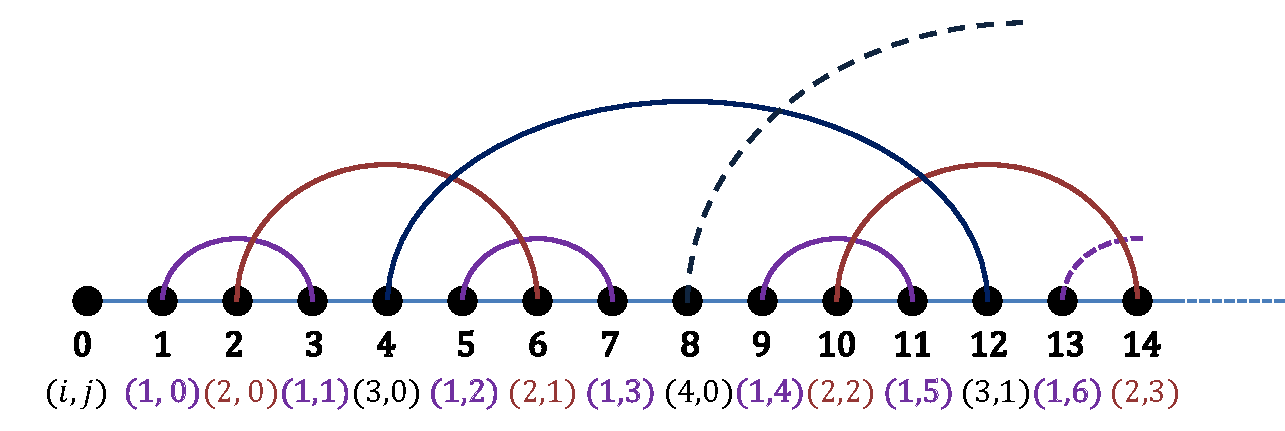
\includegraphics[width=1\columnwidth]{Chapter-1/HN3_short.pdf} 
\protect\caption{\label{fig:HN3_short} An example of the first 14 sites of HN3 on a semi-infinite line.}
\end{figure}


HN5~\cite{Boettcher09c}, as shown in Fig.~\ref{fig:Depiction-of-HN},
is an extension based on HN3, where each site in level $i$ ($i\ge2$,
i.e., all even sites) is further connected to sites that are $2^{i-1}$
sites away in both directions. For example, for the level $i=2$ sites
(sites $2,6,10,\cdots$), site 2 is connected to both site 0 and site
4; site 6 is connected to sites 4 and 8; etc. The resulting network
remains planar but has a hierarchy-dependent degree, i.e., 1/2 sites
have degree 3, 1/4 have degree 5, 1/8 have degree 7, etc. In the limit
of $N\to\infty$, this network has  average degree 5.

\begin{figure}
\centering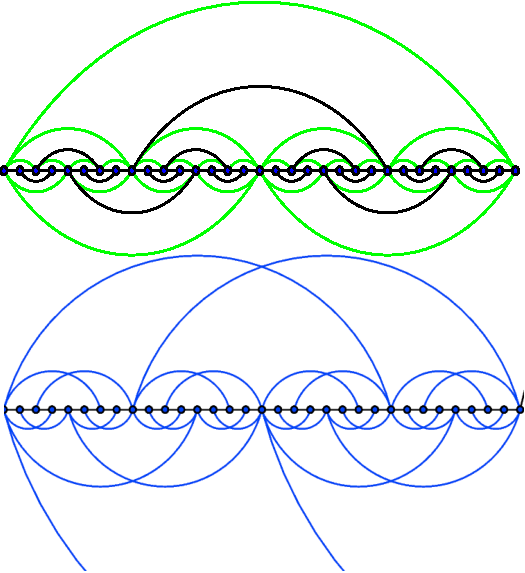
\includegraphics[width=0.8\columnwidth]{Chapter-1/HN5HNNP}
\protect\caption{\label{fig:Depiction-of-HN}Depiction of HN5 (top) and HNNP (bottom),
first introduced in Ref. \protect\cite{Boettcher09c}. Green-shaded lines
in HN5 represent its difference to HN3, which is at its core (dark
lines). While HN3 and HN5 are planar, HNNP is non-planar. }
\end{figure}

HNNP~\cite{Boettcher09c}, also shown in Fig.~\ref{fig:Depiction-of-HN},
is constructed from the same 1D backbone as HN3 and HN5. However,
for site $n$ in level $i$ with even $j$, it is connected forwards
to site $(n+3\times2^{i-1})$; while site $n$ in level $i$ with
odd $j$ is connected backwards to site $(n-3\times2^{i-1})$. Level
1 and level 2 sites have degree 3, and level $3,4,5,\cdots$ sites
have degree $5,7,9,\cdots$. The HNNP has an average degree of 4 and
is non-planar.

HN6 \cite{Boettcher09c} is constructed from HNNP in the same way of constructing HN5 from HN3. The extra links are initiated from site in level $i$ ($i\ge2$ who
i.e., all even sites)  connects to sites that are $2^{i-1}$
sites away in both directions. The resulting network is still a nonplanar with hierarchy-dependent degree.

As you can see, these four networks are all constructed hierarchically and can potentially use renormalization group in a similar way. Using these networks, renormalization group has been applied to lattice gas model \cite{cheng2015jamming, BoHa11} and ferromagnetic Ising model \cite{Boettcher2011HNNP, boettcher2015classification}. In the study here, the models are extended to lattice glass model and antiferromagnetic Ising model. 




\section{Computational Methods}
\label{sec:intro-comp}
In all the three projects in this dissertation, the computational methods are the most important part to implement the models and realize the computations. We use a wide range of different computational methods, such as Markov-Chain Monte Carlo (MCMC) method, non-Markov-Chain Monte Carlo method, Renormalization Group (RG), numerical analysis, and graphical models.
 These methods requires a broad knowledge in computer science, physics, mathematics, and statistics. Moreover, their implementations take a large amount of time and effort for coding,  testing, computation, and analysis. Our computational work may not only contribute new insights in physics but also shed light onto algorithms development and optimizations.

Specifically, we mainly adapted and implemented three advanced methods: Simulated Annealing (SA), Wang-Landau sampling (WL), and Renormalization Group (RG). 

The Simulated Annealing (SA) \cite{SA} was first formulated as an approach to find a minimization of a function with a large number of variables in statistical mechanics \cite{khachaturyan1979statistical, khachaturyan1981thermodynamic}. This algorithm imitates the slow cooling process in metallurgy to increase its crystallization and reduce its defects. In the implementation of the algorithm, it slowly decrease the probability of accepting worse transitions or solutions to robustly find a local or global minimum. In physics, the probability of a worse transition is usually controlled by the temperature, which makes this name self-explaining. Kirkpatrick {\it et. al.} \cite{SA} published a famous paper on {\it Science} to formally define, apply, and discuss SA  in the scenarios of combinatorial optimization, statistical mechanics, physics design of computer, and even the famous traveling salesman problem. It is a widely used method not only to search for a global minimum but can also to simulate the dynamics of a physical system because the annealing process simulates the physical process.
In the implementation of SA in our studies, our goal is not only simply search for the minimum (ground states) but also learn the relaxation dynamics. This process is extremely costly in terms of the computational time because we need to cool the system slowly and repeat the annealing many times ($50\sim 1000$ runs in our projects). For most SA results in Chapter 2 and 3, each curve takes about $\sim ~50$ hours using sequential computation on a single core. More detailed computing setup is described in the chapters using SA.


The Wang-Landau sampling (WL) \cite{Wang2001} is a computational methods using non-Markov-chain Monte Carlo. It is a flat histogram method which keeps track of all the random walks in the function (energy or configuration) space. Every transition from one state to another depends on all the histories of these two states. This method is based on the fact that a random walk in the function spaces with a probability proportional to the inverse of the probability density (or mass, for discrete system) enforces a flat histogram. In physics, this method is extremely attractive because it can be used to sample the density of states. Density of states can be used to calculate most physical properties using the partition function in statistical mechanics \cite{gould2010statistical}. It has been shown as a successful method in solving the problems of ferromagnetic Ising model \cite{landau2004new}, HP model of protein folding \cite{wust2008hp}, polymer chain \cite{taylor2009phase}, and numerical integration \cite{li2007numerical}. However, it has its limitations too. The two main limitations are accuracy and convergence \cite{morozov2007accuracy}. These two aspects are strongly correlated with each other and also depend on the specific problems \cite{landau2014guide, wust2008hp}. There has been a lot efforts trying to improve both aspects \cite{schulz2003avoiding, schulz2003avoiding, troster2005wang}. In our work, all the models are disordered systems with entangled geometric frustrations which makes it extremely difficult to explore all the energy or configuration space. We improved the algorithm by introducing one more type of random walk, which significantly improved the computational efficiency \cite{cheng2015jamming}. The computation time for the largest system size achieved decreases from $\sim 150$ hours to $\sim 20$ hours. More details of the setup, procedure, and results are described in Chapter 2 and 3.


The Renormalization Group (RG) \cite{wilson1975renormalization} is an analytical method to take advantage of the symmetries in the problem and to renormalize the problem to a low-dimensional self-similar one. Using RG, some problems can be solved on paper beautifully. For example, one-dimensional and two-dimensional Ising model without external magnetic fields can be solved exactly using RG \cite{onsager1944}. However, more complex problems require computational implementations using modern symbolic computational tools, such as Mathematica.  Boettcher {\it et. al.} develop a RG procedure in hierarchical networks using RG and Mathematica \cite{boettcher2012ordinary, boettcher2011rgcp, BoHa11}. We use the same RG procedure to explore various equilibrium physical properties, such as internal energy, entropy, magnetization, specific heat, susceptibility. These equilibrium results are extremely valuable to learn the dynamics and phase transitions, especially considering all computational methods may fail to equilibrate for problems of large disordered systems at low temperatures. More details of the RG setup are described in Sec. \ref{sec:afm-rg}.










